\section{The synchronized conic problem}
\label{sec:model}

\begin{definition}[Locally incompatible matching block]
For $1\le i\le m$, let
\[
 K_i=\{x_i\in\R^{n_i}_{\ge0}:A_i x_i=0\}
\]
with $A_i$ rational. A set $\mathcal F_i$ of unordered pairs of distinct coordinate indices specifies the admissible set
\[
 K_i^{\rm adm}=\{x_i\in K_i:x_{ia}x_{ib}=0\text{ for every }\{a,b\}\in\mathcal F_i\}.
\]
A rational map $P_i:\R^{n_i}\to\R^d$ is a nonnegative port map when $P_i x_i\ge0$ on $K_i$. The implementation uses the sufficient, directly checked hypothesis that every entry of $P_i$ is nonnegative.
\end{definition}

All cones are pointed because they lie in a nonnegative orthant. The feasible synchronized family is
\begin{equation}
 \mathcal X=\{(x_1,\ldots,x_m,y):x_i\in K_i^{\rm adm},\quad P_i x_i=y\ \ (1\le i\le m)\}.
 \label{eq:model}
\end{equation}
There are no additional, unrecorded cross-block conflicts. Given rational objectives $c_i,c_0$, and optional sets $Z_i$ of coordinates forced to zero, the query is whether
\begin{equation}
 \Phi(x,y)=c_0^Ty+\sum_{i=1}^m c_i^Tx_i>0
 \label{eq:objective}
\end{equation}
for some feasible tuple satisfying the zero restrictions. The zero tuple is always allowed but never answers the strict query positively.

Write $\mathcal R_i$ for the admissible extreme rays of the \emph{full} cone $K_i$, using primitive integer generators after clearing denominators. Set $R_i=|\mathcal R_i|$ and $R=\sum_iR_i$. A subset of rays is compatible when the union of their coordinate supports contains no forbidden pair. The number of local variables is $k=\max_i n_i$. The symbol $\Lambda$ denotes the full binary input length, including matrices, conflicts, dimensions and query data. Polynomial factors below may include ordinary coordinate-vector operations; they do not suppress an exponential dependence on $k$ or $d$.

\begin{lemma}[Support-respecting generation]
\label{lem:decomp}
Every admissible $x\in K_i$ is a nonnegative combination of mutually compatible rays in $\mathcal R_i$, each supported inside $\supp(x)$. The assertion remains true after arbitrary coordinate-zero restrictions.
\end{lemma}
\begin{proof}
For nonzero $x$, intersect $K_i$ with $\one^T x=1$. This is a compact rational polytope; its vertices correspond to extreme rays of $K_i$. Thus $x$ is a nonnegative combination of such rays. In a nonnegative sum, a coordinate that is zero in the sum is zero in every summand with a positive coefficient. Each participating ray is therefore supported inside $\supp(x)$. An admissible support contains no forbidden pair, so all participating rays are admissible and mutually compatible. The same argument preserves every forced zero.
\end{proof}

A useful consequence is that compatibility sectors need not be explicitly listed. One may enumerate all full-cone rays, discard inadmissible ones, and later test support unions. A face obtained by setting coordinates to zero has no new extreme rays: its rays are precisely the surviving full-cone rays. This fact is the basis of reusable anchor queries.

\subsection{Separating zero-port directions}
For a ray $r\in\mathcal R_i$, let
\[
 h_r=\one^TP_i r.
\]
Nonnegativity implies $h_r=0$ exactly when $P_i r=0$.

\begin{lemma}[Zero-port alternative]
\label{lem:zero}
If an unexcluded ray $r\in\mathcal R_i$ satisfies $h_r=0$ and $c_i^Tr>0$, then the synchronized query is positive. Otherwise, every zero-port feasible tuple has nonpositive objective, and any feasible nonzero-port tuple can be replaced, without decreasing its objective or changing its port, by one using only positive-port rays in each block.
\end{lemma}
\begin{proof}
A positive zero-port ray can be placed in its block with all other blocks zero. Conversely, decompose each local vector as in Lemma~\ref{lem:decomp}. When the total port is zero, nonnegative ray images force every participating image to be zero. By hypothesis every corresponding objective contribution is nonpositive. For a nonzero port, simply delete all zero-port ray summands. Each deletion preserves matching, admissibility, forced zeros and the port, and does not lower the objective.
\end{proof}

For the rest of the atlas construction, zero-port rays are omitted and the common port is normalized to
\[
 \Delta^{d-1}=\{y\in\R^d_{\ge0}:\one^Ty=1\}.
\]
Define the normalized source vector, port point and reward of a positive-port ray by
\begin{equation}
 v_r=r/h_r,\qquad p_r=P_i r/h_r,\qquad a_r=c_i^Tv_r.
 \label{eq:normalize}
\end{equation}
The ray's source vector and its port point must not be confused. Distinct source rays can have the same port point, different compatibility relations, and different rewards.

\section{Compatible simplices and the two-port theorem}
\label{sec:two}

\begin{lemma}[At most $d$ compatible rays at a fixed port]
\label{lem:simplex}
Suppose the positive zero-port alternative does not occur. If a block is feasible at $y\in\Delta^{d-1}$, its maximum objective at that port is attained by a convex combination of at most $d$ normalized rays. Their port points are affinely independent and their source supports are mutually compatible.
\end{lemma}
\begin{proof}
There are finitely many compatible subsets of rays. For any one such subset, the admissible coefficient vectors at port $y$ form
\[
 \{\alpha\ge0:\sum_r\alpha_rp_r=y\}.
\]
Applying $\one^T$ shows $\sum_r\alpha_r=1$, so this set is compact. The objective is $\sum_r\alpha_ra_r$. At an extreme point of the coefficient polytope, the columns $p_r$ with positive coefficients are linearly independent: otherwise a nonzero dependence permits small perturbations of both signs while keeping all positive coefficients nonnegative. There are at most $d$ such columns. Since every $p_r$ has coordinate sum one, linear independence of these columns is equivalent to affine independence of the points. Maximize over the finitely many compatible subsets and use Lemma~\ref{lem:zero} to discard nonpositive zero-port contributions.
\end{proof}

For a compatible independent set $S$, write $D_S=\conv\{p_r:r\in S\}$. At each $y\in D_S$ there is a unique barycentric expression in these points, and hence an affine reward $\ell_{i,S}(y)$. It is a function on the affine span of $D_S$; no arbitrary extension outside that span is needed. A block's optimal value is the maximum of these affine rewards over the simplexes containing $y$. The domain can be disconnected or lower-dimensional, and the maximum need not be globally concave.

\begin{theorem}[Two-port ray-image atlas]
\label{thm:two}
Let $d=2$. After checking positive zero-port rays, the strict query is decided by evaluating only the distinct normalized port points $p_r$ from all blocks. Equivalently, put
\[
 \mathcal T=\left\{\frac{(P_i r)_2}{\one^TP_i r}:r\in\mathcal R_i,\ h_r>0\right\},\qquad U=|\mathcal T|\le R.
\]
For each $t\in\mathcal T$, independently maximize the local reward among admissible single rays at slope $t$ and compatible pairs bracketing $t$. If all blocks are feasible, add their rewards and $c_0^T(1-t,t)$. The maximum over these tests equals the global normalized optimum. The same set $\mathcal T$ works for every objective and every coordinate-zero restriction.
\end{theorem}
\begin{proof}
By Lemma~\ref{lem:simplex}, local candidates are points or closed intervals with affine rewards, whose endpoints lie in $\mathcal T$. Sort the distinct slopes. Take any normalized feasible point $t$ with its maximizing local candidates. If $t\in\mathcal T$, it is already tested. Otherwise $t$ lies strictly between two consecutive slopes $u<v$. Every chosen interval containing $t$ contains all of $[u,v]$: an interval endpoint cannot lie inside $(u,v)$ by definition of consecutiveness. The chosen total reward is affine on $[u,v]$, so it is at least its value at $t$ at one endpoint. All its local candidates are feasible at that endpoint. The independently reoptimized endpoint value is no smaller.

There is no feasible point strictly outside the smallest and largest slopes, because every feasible local port is a convex combination of local ray images. Consequently no extra endpoint is required unless it is itself a ray slope. Forced zeros delete rays and candidate intervals; using the original, possibly larger slope set still refines every remaining interval. The proof never used the objective values to construct $\mathcal T$.
\end{proof}

\begin{remark}[Why reward-line intersections are unnecessary]
On an open interval between consecutive domain endpoints, the available local affine pieces are fixed. Their pointwise maxima, and the sum of these maxima, are convex there. Maximizing such a function needs only the interval endpoints. The proof above is stronger than an appeal to global convexity: it remains valid when new pieces appear only at an endpoint or when the feasible set is disconnected. It is the endpoints of \emph{domains}, not crossings of reward lines, that matter.
\end{remark}

For normalized ray slopes $s<t$ with rewards $a_s,a_t$, the reward at $u\in[s,t]$ is
\[
 \frac{t-u}{t-s}a_s+\frac{u-s}{t-s}a_t.
\]
Pairs with equal slopes never improve on the better singleton. They need not be mixed, especially when their source supports are incompatible.

\begin{corollary}[Direct two-port cost]
\label{cor:two-cost}
After local rays are known, preparation and one query require at most
\[
 O\!\left(U\sum_{i=1}^m(R_i+R_i^2)\right)
\]
exact rational operations, apart from sorting, coordinate-support work and polynomial-size linear-algebra factors. Barycentric mixtures may be cached once and reused for arbitrarily many objectives and coordinate-zero faces.
\end{corollary}
\begin{proof}
There are at most $R_i$ singleton candidates and $\binom{R_i}{2}$ pair candidates in block $i$. At each of the $U$ slopes, test interval membership, compatibility and the affine reward. Caching their coefficients removes repeated interpolation from later queries. All tests use exact rational comparisons.
\end{proof}

\section{A finite atlas in every port dimension}
\label{sec:atlas}
The two-port theorem does not extend by keeping only ray images. In three ports, two feasible line segments can meet at a point that is a ray image of neither block. An arrangement of simplex boundary hyperplanes captures the missing points without introducing objective-dependent walls.

\subsection{The coordinate-frame construction}
Let $E=\{e_1,\ldots,e_d\}$ be the standard coordinate frame. In each block, combine its distinct positive-port points with $E$. For every linearly independent $(d-1)$-subset of this set, retain the hyperplane through its span. Let $\mathcal H$ be the union of these hyperplanes over all blocks, with duplicates removed. Hyperplanes are stored by primitive integer normal vectors, up to sign.

The frame ensures that $\mathcal H$ contains $y_j=0$ for every $j$. Define $\mathcal V$ to consist of all points of $\Delta^{d-1}$ obtained as a unique intersection of $\one^Ty=1$ and $d-1$ hyperplanes in $\mathcal H$. For $d=1$, define $\mathcal V=\{(1)\}$. Hyperplanes whose normals are dependent, inconsistent intersection systems, and intersections outside the nonnegative simplex are discarded by exact arithmetic.

\begin{lemma}[Every compatible simplex is an arrangement subcomplex]
\label{lem:frame}
Every $D_S$ is a union of closed cells of the hyperplane arrangement $\mathcal H$ inside $\Delta^{d-1}$. This includes simplexes of all dimensions, not just full-dimensional ones.
\end{lemma}
\begin{proof}
Suppose $S$ has $r\le d$ independent port columns $p_1,\ldots,p_r$. Complete these columns to a basis of $\R^d$ by choosing $d-r$ vectors from $E$; this is possible because $E$ spans the ambient space. Write the resulting basis as
\[
 B=(p_1,\ldots,p_r,e_{j_1},\ldots,e_{j_{d-r}}).
\]
In the corresponding basis coordinates, membership in $D_S$ means that the last $d-r$ coordinates vanish, the first $r$ are nonnegative, and the ambient normalization holds. When the last coordinates vanish, normalization makes the sum of the first $r$ coordinates equal one because each $p_i$ has coordinate sum one.

The vanishing hyperplane for each basis coordinate is spanned by the other $d-1$ basis vectors. All these vectors come from the same local point set together with $E$, so every such hyperplane belongs to $\mathcal H$. Thus the affine-span equations and all supporting facets of $D_S$ are arrangement hyperplanes. On a relatively open arrangement cell, all their signs are fixed. If one point of that cell lies in $D_S$, the whole cell does; its closure lies there as well because $D_S$ is closed. This proves the assertion.
\end{proof}

\begin{theorem}[Universal projective atlas]
\label{thm:atlas}
After the zero-port alternative is checked, the maximum of every normalized synchronized objective is attained at a point of $\mathcal V$, whenever a nonzero port is feasible. The set $\mathcal V$ depends only on the local cones, conflicts and port maps. It remains complete for every collection of coordinate-zero restrictions.
\end{theorem}
\begin{proof}
By the preceding lemmas, the normalized feasible set is a finite union of intersections of compatible local simplexes. These are compact. On each such intersection, the selected total reward is affine; hence a finite global maximum exists whenever the feasible set is nonempty.

Alternatively, start with any feasible tuple, remove nonpositive zero-port summands, and choose maximizing compatible simplex representations at its port $y$. Let $C$ be the relatively open arrangement cell containing $y$. By Lemma~\ref{lem:frame}, every chosen simplex contains $\overline C$. The chosen total reward is affine on this compact polytope, so one of its vertices $v$ has reward at least the reward at $y$. Reoptimizing the blocks at $v$ can only increase that value.

Every vertex of an arrangement cell in the $(d-1)$-dimensional affine space $\one^Ty=1$ is specified by $d-1$ independent active arrangement hyperplanes, including coordinate hyperplanes when necessary. Thus $v\in\mathcal V$. Lower-dimensional cells are covered by the same argument. Setting source coordinates to zero merely deletes rays and simplexes, and the original arrangement still refines each surviving simplex. No objective coefficient was used in constructing the arrangement.
\end{proof}

\subsection{The three-port intersection example}
\begin{example}[A required point absent from all ray images]
\label{ex:centroid}
Take two two-ray orthant blocks with no conflicts. Their integer port columns are
\[
 P_1=((2,0,0)^T,(0,1,1)^T),\qquad
 P_2=((0,2,0)^T,(1,0,1)^T).
\]
Their normalized domains are the medians joining $e_1$ to $(e_2+e_3)/2$ and $e_2$ to $(e_1+e_3)/2$. Their intersection is the singleton
\[
 y_*=(1/3,1/3,1/3).
\]
It is not a local ray image, but it is an arrangement vertex. For objective one on every source coordinate, the total normalized reward is one. An atlas restricted to ray images would falsely report no nonzero common port.
\end{example}

\begin{figure}[ht]
\centering
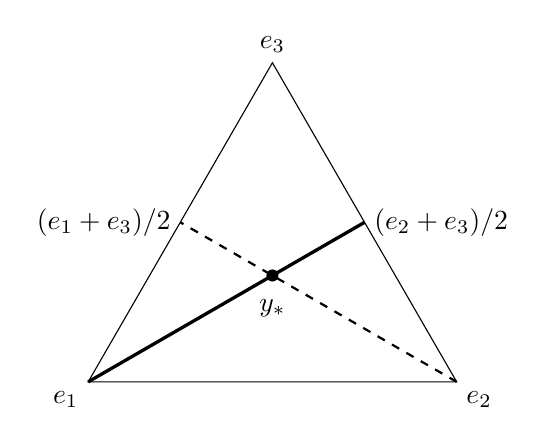
\begin{tikzpicture}[scale=.78]
\coordinate (A) at (0,0);\coordinate (B) at (6,0);\coordinate (C) at (3,5.196);
\coordinate (D) at (4.5,2.598);\coordinate (E) at (1.5,2.598);\coordinate (G) at (3,1.732);
\draw (A)--(B)--(C)--cycle;
\draw[very thick] (A)--(D);\draw[thick,dashed] (B)--(E);
\fill (G) circle (2.8pt);
\node[below left] at (A) {$e_1$};\node[below right] at (B) {$e_2$};\node[above] at (C) {$e_3$};
\node[right] at (D) {$(e_2+e_3)/2$};\node[left] at (E) {$(e_1+e_3)/2$};
\node[below,yshift=-5pt] at (G) {$y_*$};
\end{tikzpicture}
\caption{The two blocks are feasible on the solid and dashed medians, respectively. Their only common normalized port is a new intersection point. The figure concerns exact rational domains, not a geometric normal-surface embedding.}
\end{figure}

\section{Complete enumeration and binary complexity}
\label{sec:complexity}

\subsection{A deliberately simple complete local enumerator}
\begin{proposition}[Support characterization of rays]
\label{prop:support}
For a nonzero $x\in K_i$ with support $S$, its ray is extreme in $K_i$ exactly when
\[
 \dim\ker(A_i|_S)=1.
\]
Consequently, enumerating all nonempty coordinate supports, checking compatibility, testing one-dimensional nullity, and retaining the strictly positive kernel generators produces every admissible extreme ray exactly once.
\end{proposition}
\begin{proof}
If the support kernel has dimension greater than one, choose a vector in it not proportional to $x$. Sufficiently small perturbations of both signs remain positive on $S$ and zero elsewhere; they express $x$ as a nontrivial average of nonproportional cone vectors. Conversely, if $x=u+v$ with $u,v\ge0$ in the kernel, both $u,v$ are supported in $S$. One-dimensional nullity makes them nonnegative multiples of $x$. The support of a strictly positive kernel generator is exactly $S$, so distinct accepted supports cannot duplicate a ray.
\end{proof}

This costs $2^{n_i}\poly(\Lambda)$ bit operations by exact rational elimination, and gives $R_i\le2^{n_i}-1$. It is not asserted to outperform every established normal-surface enumerator. Its purpose is a transparent complete baseline with explicit cost, which can later be replaced by a faster producer without changing the atlas theorem.

\subsection{A nullity-sensitive alternative for long blocks}
Small coordinate count is not the only useful local parameter. Let
\[
 h_i=n_i-\rank A_i.
\]
When $h_i=0$ there are no nonzero local vectors. For $h_i\ge1$, consider all sets of $h_i-1$ coordinates to be set to zero. Restrict $A_i$ to the remaining coordinates. If its kernel is one-dimensional and has a nonnegative generator, restore the omitted zeros, check compatibility, and deduplicate the primitive ray.

\begin{proposition}[Zero-set enumerator]
\label{prop:zeros}
The procedure above enumerates precisely the admissible extreme rays and uses
\[
 \binom{n_i}{h_i-1}\poly(\Lambda)
\]
bit operations. In particular, $R_i\le\binom{n_i}{h_i-1}$. This is a standard active-coordinate method, included here as a compatible local producer rather than claimed as a new enumeration principle.
\end{proposition}
\begin{proof}
Every accepted vector has one-dimensional support kernel, possibly after additional zeros arise within the retained coordinates, so Proposition~\ref{prop:support} proves extremality. Conversely, let $r$ be an extreme ray and let $Z$ be its zero coordinates. Restricting the coordinate functionals in $Z$ to $\ker A_i$ cuts its dimension from $h_i$ to one. Choose $h_i-1$ independent functionals from those restrictions. The corresponding candidate zero set leaves exactly the ray line in the kernel and therefore recovers $r$. Rational nullspace computation and primitive scaling have polynomial bit cost. Duplicate zero sets may recover the same ray, which the implementation removes by an exact set of integer tuples.
\end{proof}

The delivery implements this as \code{enumerate_rays_by_zeros}, selected by \code{Prepared(..., ray_method='zeros')}. The default remains the support method: fewer combinatorial candidates need not mean less Python time, since early compatibility rejection and matrix sizes differ. The reported paired benchmarks use the same default support enumerator on both sides. The alternative is independently cross-checked on all random local blocks and on a 40-variable nullity-one chain.

\subsection{Counting hyperplanes, vertices and simplexes}
Let $U$ be the number of distinct normalized port points across all blocks. For $d\ge2$,
\begin{equation}
 H:=|\mathcal H|\le\binom{U+d}{d-1},\qquad
 |\mathcal V|\le\binom H{d-1}.
 \label{eq:counts}
\end{equation}
The first bound deliberately overcounts: our construction uses block-local subsets, while the right side allows subsets from the entire union. There are at most
\[
 S_i\le\sum_{j=1}^{\min(d,R_i)}\binom{R_i}{j}
\]
compatible independent candidates in block $i$. Direct enumeration of arrangement vertices, followed by all local simplex membership tests at those vertices, therefore uses
\begin{equation}
 \poly(\Lambda,d)\,(R+d+1)^{(d-1)^2+d}
 =\poly(\Lambda,d)\,(R+d+1)^{d^2-d+1}
 \label{eq:ray-cost}
\end{equation}
bit operations, once the rays are available. The same bound accommodates constructing and caching the barycentric tables. A memory-saving variant enumerates vertices and local candidates on demand rather than storing every mixture. The shipped implementation favors reusable tables for repeated objectives.

\begin{lemma}[Polynomial bit size of arithmetic objects]
\label{lem:bits}
Primitive local ray coordinates, normalized port points, hyperplane normals, atlas vertices, barycentric weights, and assembled witnesses all have bit length polynomial in the encoded input and in $d$. The number of objects may be exponential, but no single object needs exponentially many bits merely because many alternatives were enumerated.
\end{lemma}
\begin{proof}
Clear denominators of input rows. Their resulting coefficient bit lengths remain polynomial in the original input length. A one-dimensional support kernel has a generator given by minors of an independent subsystem. Hadamard's inequality bounds the logarithms of these minors by a polynomial in the support size and coefficient bits. Port multiplication, summation and normalization preserve polynomial bit size.

Hyperplane normals are minors of matrices with at most $d-1$ normalized port rows. Atlas vertices and barycentric weights are solutions of systems of order at most $d$, so the same determinant argument applies. An assembled local vector is a sum of at most $d$ weighted normalized rays. Summing the polynomially many local objective contributions increases bit length by at most a polynomial factor. All coefficients used for these constructions come from the source and the chosen finite index sets; there is no unbounded-depth chain of arithmetic substitutions.
\end{proof}

\begin{theorem}[Implemented parameter bound]
\label{thm:cost}
The complete support enumerator and direct atlas algorithm decide \eqref{eq:objective}, with exact witnesses for positive answers, in
\begin{equation}
 \poly(\Lambda,d)\exp\!\left(O\bigl(d^2(k+\log(m+d+2))\bigr)\right)
 \label{eq:cost}
\end{equation}
bit time. For fixed $d$, this is polynomial in $m$ and singly exponential in $k$. If $\Lambda$ is polynomial in $N$ and $d,k=O(\log N)$, it is $2^{O((\log N)^3)}$.
\end{theorem}
\begin{proof}
Local enumeration costs $m2^k\poly(\Lambda)$. Moreover $R\le m2^k$, so the logarithm of \eqref{eq:ray-cost} is
\[
 O\bigl((d^2-d+1)\log(R+d+1)\bigr)
 =O\bigl(d^2(k+\log(m+d+2))\bigr).
\]
Lemma~\ref{lem:bits} justifies the bit-cost rather than unit-cost interpretation. The claimed specializations follow by substitution. For $d=1$, the one-point atlas and singleton local candidates give the same bound directly.
\end{proof}

\begin{corollary}[Large blocks with bounded nullity]
\label{cor:nullity}
Suppose $\Lambda$ and $m$ are polynomial in $N$, the local nullities $h_i$ are bounded by an absolute constant, and $d=O(\log N)$. The implemented zero-set producer followed by the atlas algorithm solves the discovery problem in $2^{O((\log N)^3)}$ bit time, without requiring $n_i=O(\log N)$.
\end{corollary}
\begin{proof}
Proposition~\ref{prop:zeros} gives polynomial local preparation time and polynomial $R$. Apply \eqref{eq:ray-cost}. The exponent is $O(d^2\log N)=O((\log N)^3)$.
\end{proof}

This alternative matters for long pieces whose matching data have few genuine degrees of freedom. It does not assert that unrestricted normal matching blocks always have small nullity. Source-verified sector restrictions or exact compression must justify any such application.

The support and atlas caps in the code raise \code{ResourceLimit}. They are not proofs of nonexistence. A complete negative answer is returned only after all required local supports and atlas candidates have been processed. Positive packets are independently checkable; this package does not supply a short independently replayable certificate of a negative optimum.

\subsection{Signed ports: a proved extension}
\begin{corollary}[Orthant lifting]
\label{cor:signed}
The discovery problem with arbitrary rational signed common port maps reduces to at most $2^d$ nonnegative-port problems, each with $n_i+d$ variables in block $i$. Thus the same type of bound holds with $k$ replaced by $k+d$ and a further factor $2^d$.
\end{corollary}
\begin{proof}
Choose a common sign vector $\sigma\in\{-1,1\}^d$. Adjoin nonnegative local coordinates $z_i$ and equations
\[
 P_i x_i=\operatorname{diag}(\sigma)z_i.
\]
Use $z_i$ as the new port, synchronize all copies, retain the original conflicts on $x_i$, and put zero local objective on the added coordinates. The master objective becomes $c_0^T\operatorname{diag}(\sigma)z$. Every signed port belongs to at least one closed orthant, including ports with zero coordinates, and the lifting is exact in each orthant. The new port map is a coordinate projection and therefore entrywise nonnegative.
\end{proof}

This extension is proved, not exposed as a separate implemented backend in the delivery. Its new local cone rays must be enumerated after lifting: sign inequalities need not be coordinate faces of the original cone. Reusing only the original rays would be an unjustified shortcut.
